\documentclass[12pt,a4paper]{article}

% ─── Page Layout ───────────────────────────────────────────────────────────────
\usepackage[a4paper, margin=0.8in, headheight=14pt]{geometry}

% ─── Fonts (XeLaTeX) ───────────────────────────────────────────────────────────
\usepackage{fontspec}
\usepackage{unicode-math}
\setmainfont{TeX Gyre Pagella}
\setmonofont[Scale=0.88]{TeX Gyre Cursor}
\setmathfont{Latin Modern Math}

% ─── Packages ──────────────────────────────────────────────────────────────────
\usepackage{xcolor}
\usepackage{colortbl}
\usepackage{titlesec}
\usepackage{enumitem}
\usepackage{tabularx}
\usepackage{booktabs}
\usepackage{array}
\usepackage{amsmath}
\usepackage{tikz}
\usetikzlibrary{shapes.geometric, arrows.meta, positioning, calc, fit, decorations.pathreplacing}
\usepackage{tcolorbox}
\tcbuselibrary{skins, breakable}
\usepackage{hyperref}
\usepackage{fancyhdr}
\usepackage{graphicx}
\usepackage{microtype}
\hyphenpenalty=10000
\exhyphenpenalty=10000
\sloppy
\usepackage{caption}
\usepackage{setspace}
\usepackage{multirow}
\usepackage{tocloft}

% ─── Q&A helper ────────────────────────────────────────────────────────────────
\newcommand{\Q}[1]{\textbf{#1}\par\noindent\ignorespaces}

% ─── Colour Palette ────────────────────────────────────────────────────────────
\definecolor{myred}{RGB}{196,30,58}
\definecolor{mydark}{RGB}{30,30,50}
\definecolor{mygreen}{RGB}{14,120,80}
\definecolor{myteal}{RGB}{0,130,140}
\definecolor{myamber}{RGB}{180,100,0}
\definecolor{mypurple}{RGB}{100,30,160}
\definecolor{mygray}{RGB}{246,247,249}
\definecolor{mgframe}{RGB}{180,185,200}
\definecolor{watermark}{RGB}{145,150,170}
\definecolor{hdrred}{RGB}{250,232,235}
\definecolor{hdrgreen}{RGB}{220,244,233}
\definecolor{hdrteal}{RGB}{220,242,244}
\definecolor{hdramber}{RGB}{253,242,215}
\definecolor{hdrpurple}{RGB}{238,228,255}
\definecolor{hdrgray}{RGB}{238,240,245}
\definecolor{rowalt}{RGB}{250,251,253}

% ─── Section Formatting ────────────────────────────────────────────────────────
\titleformat{\section}
  {\large\bfseries\color{myred}}{\thesection.}{0.5em}{}
  [\vspace{1pt}{\color{myred}\rule{\linewidth}{0.8pt}}]
\titleformat{\subsection}
  {\normalsize\bfseries\color{myteal}}{\thesubsection}{0.5em}{}
\titlespacing*{\section}{0pt}{18pt}{7pt}
\titlespacing*{\subsection}{0pt}{11pt}{4pt}

% ─── Paragraph ─────────────────────────────────────────────────────────────────
\setlength{\parindent}{0pt}
\setlength{\parskip}{4pt}

% ─── TOC Styling ───────────────────────────────────────────────────────────────
\renewcommand{\cfttoctitlefont}{\large\bfseries\color{myred}}
\renewcommand{\cftaftertoctitle}{\par\noindent{\color{myred}\rule{\linewidth}{0.8pt}}}
\setlength{\cftbeforetoctitleskip}{0pt}
\setlength{\cftaftertoctitleskip}{6pt}
\renewcommand{\cftsecfont}{\normalsize\bfseries\color{mydark}}
\renewcommand{\cftsecpagefont}{\normalsize\bfseries\color{mydark}}
\renewcommand{\cftsecleader}{\cftdotfill{\cftdotsep}}
\setlength{\cftbeforesecskip}{7pt}
\renewcommand{\cftsubsecfont}{\small\color{mydark}}
\renewcommand{\cftsubsecpagefont}{\small\color{mydark}}
\setlength{\cftbeforesubsecskip}{3pt}
\setlength{\cftsubsecindent}{1.4em}

% ─── Table helpers ─────────────────────────────────────────────────────────────
\renewcommand{\arraystretch}{1.45}
\setlength{\tabcolsep}{6pt}
\arrayrulecolor{mydark}
\newcolumntype{B}[1]{>{\small\bfseries\raggedright\arraybackslash}m{#1}}
\newcolumntype{Y}{>{\small\raggedright\arraybackslash}X}
\renewcommand{\tabularxcolumn}[1]{m{#1}}

% ─── Header / Footer ───────────────────────────────────────────────────────────
\pagestyle{fancy}
\fancyhf{}
\fancyhead[L]{\small\color{myred}\textbf{EC301}\;\color{mydark}--- Electronic Devices}
\fancyhead[R]{\small\color{myteal}\textbf{Module 3 Notes}}
\fancyfoot[C]{\small\color{mydark}\thepage}
\fancyfoot[R]{\small\color{watermark}\textit{\copyright\ Biraj}}
\renewcommand{\headrulewidth}{0.5pt}
\renewcommand{\footrulewidth}{0.3pt}

% ─── Hyperref ──────────────────────────────────────────────────────────────────
\hypersetup{
  colorlinks=true, linkcolor=myteal, urlcolor=myteal,
  pdfauthor={Biraj Sarkar (CGEC)},
  pdftitle={EC301 --- Module 3 Notes: MOSFET Physics, C-V and Small Signal Models}
}

% ─── tcolorbox styles ──────────────────────────────────────────────────────────
\tcbset{
  tikzbox/.style={
    colback=mygray, colframe=mgframe, boxrule=0.6pt, arc=4pt,
    left=8pt, right=8pt, top=6pt, bottom=6pt,
    colbacktitle=mgframe, coltitle=mydark,
    fonttitle=\small\bfseries
  },
  defbox/.style={
    colback=hdrgreen, colframe=mygreen, boxrule=0.8pt, arc=4pt,
    left=9pt, right=9pt, top=6pt, bottom=6pt,
    colbacktitle=mygreen, coltitle=white,
    fonttitle=\small\bfseries
  },
  formulabox/.style={
    colback=hdrteal, colframe=myteal, boxrule=0.8pt, arc=4pt,
    left=9pt, right=9pt, top=7pt, bottom=7pt,
    colbacktitle=myteal, coltitle=white,
    fonttitle=\small\bfseries
  },
  examplebox/.style={
    colback=hdramber, colframe=myamber, boxrule=0.8pt, arc=4pt,
    left=9pt, right=9pt, top=6pt, bottom=6pt,
    colbacktitle=myamber, coltitle=white,
    fonttitle=\small\bfseries
  },
  masonbox/.style={
    colback=hdrpurple, colframe=mypurple, boxrule=0.8pt, arc=4pt,
    left=9pt, right=9pt, top=6pt, bottom=6pt,
    colbacktitle=mypurple, coltitle=white,
    fonttitle=\small\bfseries
  },
  exambox/.style={
    colback=hdrpurple, colframe=mypurple, boxrule=1pt, arc=5pt,
    left=10pt, right=10pt, top=8pt, bottom=8pt,
    colbacktitle=mypurple, coltitle=white,
    fonttitle=\bfseries,
    breakable, title after break={\textbf{Frequently Asked / Viva Questions (contd.)}}}
}
\tcbset{breakable}

% ─── TikZ styles ───────────────────────────────────────────────────────────────
\tikzset{
  block/.style={rectangle, draw=myteal, fill=hdrteal,
    text width=2.4cm, align=center, minimum height=0.95cm,
    font=\small, rounded corners=3pt, line width=0.7pt},
  redblock/.style={rectangle, draw=myred, fill=hdrred,
    text width=2.4cm, align=center, minimum height=0.95cm,
    font=\small, rounded corners=3pt, line width=0.7pt},
  greenblock/.style={rectangle, draw=mygreen, fill=hdrgreen,
    text width=2.4cm, align=center, minimum height=0.95cm,
    font=\small, rounded corners=3pt, line width=0.7pt},
  amberblock/.style={rectangle, draw=myamber, fill=hdramber,
    text width=2.4cm, align=center, minimum height=0.95cm,
    font=\small, rounded corners=3pt, line width=0.7pt},
  purpblock/.style={rectangle, draw=mypurple, fill=hdrpurple,
    text width=2.4cm, align=center, minimum height=0.95cm,
    font=\small, rounded corners=3pt, line width=0.7pt},
  arrow/.style={-Stealth, thick, color=mydark},
  redarrow/.style={-Stealth, thick, color=myred},
  line/.style={thick, color=mydark}
}

% ═══════════════════════════════════════════════════════════════════════════════
\begin{document}
% ═══════════════════════════════════════════════════════════════════════════════

\begin{center}
  {\LARGE\bfseries\color{myred} EC301 --- Electronic Devices}\\[5pt]
  {\normalsize\color{mydark} Semester III \quad$\bullet$\quad 3L:0T:0P \quad$\bullet$\quad 3 Credits}\\[3pt]
  {\normalsize\color{myteal}\textbf{Module 3 Exam Notes: MOSFET Physics, C-V \& Small Signal Models}}\\[3pt]
  {\small\color{mydark} CGEC \;$|$\; B.Tech ECE (2023--27) \;$|$\; \textit{Biraj Sarkar}}
\end{center}
\vspace{2pt}
\noindent{\color{myred}\rule{\linewidth}{1.5pt}}
\vspace{2pt}

\hypersetup{linkcolor=mydark}
\tableofcontents
\hypersetup{linkcolor=myteal}
\newpage

% ===============================================================================
\section{The MOS Capacitor Physics and Energy Bands}
% ===============================================================================

The \textbf{Metal-Oxide-Semiconductor (MOS) capacitor} is the fundamental two-terminal building block of all MOS Field-Effect Transistors. It consists of a top metal (or heavily doped polycrystalline silicon) gate electrode, an insulating silicon dioxide ($\text{SiO}_2$) layer of thickness $t_{ox}$, and a semiconductor silicon substrate.

\subsection{Basic Structure and Flat-Band Condition}
Consider an ideal MOS capacitor on a p-type Silicon substrate with acceptor doping $N_A$:
\begin{itemize}[leftmargin=*, itemsep=3pt]
  \item \textbf{Oxide Capacitance per unit area ($C_{ox}$):}
  \begin{equation}
    C_{ox} = \frac{\epsilon_{ox}}{t_{ox}}
  \end{equation}
  where $\epsilon_{ox} = \epsilon_r \epsilon_0 \approx 3.9 \times 8.854 \times 10^{-14}\,\text{F/cm} \approx 3.45 \times 10^{-13}\,\text{F/cm}$.
  \item \textbf{Flat-Band Voltage ($V_{FB}$):} Due to the difference in work function between the gate metal $\Phi_m$ and semiconductor $\Phi_s$ ($\Phi_{ms} = \Phi_m - \Phi_s$), and fixed positive charges trapped inside the oxide or at the oxide-semiconductor interface ($Q_{ox}$), the energy bands are bent even at zero gate bias ($V_G = 0$). The specific external gate voltage that restores flat energy bands up to the interface ($\psi_s = 0$) is the \textbf{flat-band voltage}:
  \begin{equation}
    V_{FB} = \Phi_{ms} - \frac{Q_{ox}}{C_{ox}}
  \end{equation}
\end{itemize}

\subsection{Three Surface Charge Regimes of the MOS Capacitor}
As the gate voltage $V_G$ varies relative to $V_{FB}$, the surface potential $\psi_s$ at the $\text{Si}\text{--}\text{SiO}_2$ interface changes, establishing three distinct operating regimes:

\begin{enumerate}[label=\arabic*., leftmargin=*]
  \item \textbf{Accumulation ($V_G < V_{FB}$ for p-substrate):}
  A negative gate voltage bends the energy bands upward at the interface ($\psi_s < 0$), pulling the valence band edge $E_v$ closer to the Fermi level $E_F$. Majority holes accumulate at the silicon surface, forming a thin sheet of positive mobile hole charge ($Q_s > 0$).

  \item \textbf{Depletion ($V_{FB} < V_G < V_T$ for p-substrate):}
  A positive gate voltage bends the energy bands downward ($\psi_s > 0$), pushing majority holes away from the surface into the bulk. This leaves behind an uncompensated, immobile space charge layer of ionized acceptor atoms ($-q N_A$) of depletion width $W$:
  \begin{equation}
    W = \sqrt{\frac{2 \epsilon_s \psi_s}{q N_A}}
  \end{equation}
  The depletion charge per unit area is $Q_d = -q N_A W = -\sqrt{2 q \epsilon_s N_A \psi_s}$.

  \item \textbf{Inversion ($V_G \ge V_T$ for p-substrate):}
  As $V_G$ increases further, the bands bend downward so severely that the intrinsic Fermi level $E_i$ crosses below the Fermi level $E_F$ at the interface.
  \begin{itemize}
    \item \textbf{Onset of Weak Inversion:} Occurs when $E_i$ crosses $E_F$ at the surface ($\psi_s = \phi_F$), where $\phi_F = V_T \ln(N_A / n_i)$ is the bulk potential. The surface becomes n-type ($n_s > p_s$).
    \item \textbf{Threshold / Strong Inversion ($\psi_s = 2\phi_F$):} The electron concentration at the surface equals the original bulk hole concentration: $n_s = N_A$. An extremely thin ($< 5\text{--}10\,\text{nm}$) and highly conductive layer of minority electrons (the \textbf{inversion layer}) forms directly beneath the oxide.
  \end{itemize}
\end{enumerate}

\begin{tcolorbox}[tikzbox, title={Energy Band Diagram of MOS Capacitor on P-Substrate in Inversion}]
\centering
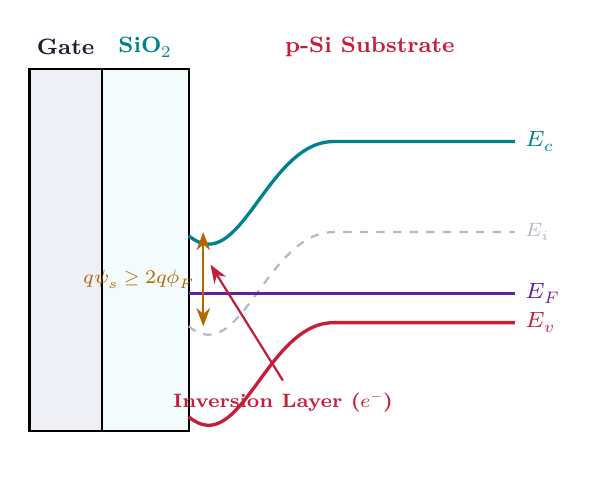
\begin{tikzpicture}[scale=0.92]
  % Regions: Metal | Oxide | Silicon
  \draw[thick, fill=hdrgray] (-3.2, -1.5) rectangle (-2.2, 3.5);
  \node[font=\footnotesize\bfseries\color{mydark}] at (-2.7, 3.8) {Gate};

  \draw[thick, fill=hdrteal!30] (-2.2, -1.5) rectangle (-1.0, 3.5);
  \node[font=\footnotesize\bfseries\color{myteal}] at (-1.6, 3.8) {$\text{SiO}_2$};

  \node[font=\footnotesize\bfseries\color{myred}] at (1.5, 3.8) {p-Si Substrate};

  % Energy bands in Silicon
  % Ec bending down
  \draw[very thick, color=myteal] (-1.0, 1.2) to[out=-40, in=180] (1.0, 2.5) -- (3.5, 2.5) node[right, font=\footnotesize\bfseries] {$E_c$};
  % Ev bending down
  \draw[very thick, color=myred] (-1.0, -1.3) to[out=-40, in=180] (1.0, 0.0) -- (3.5, 0.0) node[right, font=\footnotesize\bfseries] {$E_v$};
  % Ei dashed bending down
  \draw[dashed, thick, color=mgframe] (-1.0, -0.05) to[out=-40, in=180] (1.0, 1.25) -- (3.5, 1.25) node[right, font=\scriptsize] {$E_i$};

  % EF flat horizontal
  \draw[very thick, color=mypurple] (-1.0, 0.4) -- (3.5, 0.4) node[right, font=\footnotesize\bfseries] {$E_F$};

  % Potential indicators
  \draw[Stealth-Stealth, thick, color=myamber] (-0.8, -0.05) -- (-0.8, 1.25) node[midway, left, font=\scriptsize\bfseries] {$q\psi_s \ge 2q\phi_F$};
  \node[font=\scriptsize\bfseries\color{myred}] at (0.3, -1.1) {Inversion Layer ($e^-$)};
  \draw[-Stealth, thick, color=myred] (0.3, -0.8) -- (-0.7, 0.8);
\end{tikzpicture}
\end{tcolorbox}

\subsection{Threshold Voltage Derivation}
At the onset of strong inversion ($\psi_s = 2\phi_F$), the depletion region reaches its maximum width $W_{\text{max}}$:
\begin{equation}
  W_{\text{max}} = \sqrt{\frac{4 \epsilon_s \phi_F}{q N_A}}
\end{equation}
Beyond this point, any further increase in gate voltage is shielded by the exponentially growing inversion electron charge, locking the depletion width at $W_{\text{max}}$. The maximum depletion charge per unit area is:
\begin{equation}
  Q_{d,\text{max}} = -q N_A W_{\text{max}} = -\sqrt{4 q \epsilon_s N_A \phi_F}
\end{equation}

By voltage loop across the MOS structure, the applied gate threshold voltage $V_T$ is:
\begin{equation}
  V_T = V_{FB} + V_{ox} + \psi_s = V_{FB} - \frac{Q_{d,\text{max}}}{C_{ox}} + 2\phi_F
\end{equation}

\begin{tcolorbox}[formulabox, title={\textbf{Threshold Voltage and Body Effect Equations}}]
\begin{equation}
  V_{T0} = V_{FB} + 2\phi_F + \frac{\sqrt{4 q \epsilon_s N_A \phi_F}}{C_{ox}}
\end{equation}
When a reverse substrate-to-source body bias ($V_{SB} > 0$) is applied:
\begin{equation}
  V_T = V_{T0} + \gamma \left(\sqrt{2\phi_F + V_{SB}} - \sqrt{2\phi_F}\right)
\end{equation}
where $\gamma$ is the \textbf{body effect coefficient}:
\begin{equation}
  \gamma = \frac{\sqrt{2 q \epsilon_s N_A}}{C_{ox}} \quad (\text{V}^{1/2})
\end{equation}
\end{tcolorbox}

% ===============================================================================
\section{C-V Characteristics of the MOS Capacitor}
% ===============================================================================

The capacitance of an MOS capacitor is defined as $C = dQ_G / dV_G$. The total capacitance is the series combination of the fixed oxide capacitance $C_{ox}$ and the semiconductor surface capacitance $C_s$:

\begin{equation}
  C = \frac{C_{ox} C_s}{C_{ox} + C_s}
\end{equation}

\par\vspace{6pt}\noindent
\begingroup
\setlength{\tabcolsep}{5pt}
\setlength{\extrarowheight}{3pt}
\renewcommand{\arraystretch}{1.35}
\begin{tabularx}{\linewidth}{|B{2.8cm}|Y|Y|}
\hline
\multicolumn{1}{|c|}{\textbf{Bias Regime}} & \multicolumn{1}{c|}{\textbf{Low-Frequency (LF) Capacitance}} & \multicolumn{1}{c|}{\textbf{High-Frequency (HF) Capacitance}} \\
\hline
Accumulation ($V_G < V_{FB}$) & $C = C_{ox}$ \newline Majority holes accumulate immediately at interface ($C_s \to \infty$). & $C = C_{ox}$ \newline Majority holes respond rapidly up to multi-GHz frequencies. \\
\hline
Depletion ($V_{FB} < V_G < V_T$) & $C = \frac{C_{ox} C_{\text{dep}}}{C_{ox} + C_{\text{dep}}} < C_{ox}$ \newline Decreases monotonically as depletion layer widens ($W \propto \sqrt{\psi_s}$). & $C = \frac{C_{ox} C_{\text{dep}}}{C_{ox} + C_{\text{dep}}} < C_{ox}$ \newline Depletion layer capacitance dominates identically for LF and HF. \\
\hline
Strong Inversion ($V_G \ge V_T$) & $C = C_{ox}$ \newline Thermal generation-recombination ($1\text{--}100\,\text{Hz}$) keeps pace with slow AC signal; inversion charge $Q_n$ modulates. & $C = C_{\text{min}} = \frac{C_{ox} C_{\text{dep,max}}}{C_{ox} + C_{\text{dep,max}}}$ \newline Minority carriers cannot respond ($f \ge 100\,\text{kHz}$); depletion layer stays locked at $W_{\text{max}}$. \\
\hline
Deep Depletion (Fast Ramp) & Not observed under slow quasi-static sweeps. & $C$ continues to decrease below $C_{\text{min}}$ because inversion layer has no time to generate; $W > W_{\text{max}}$. \\
\hline
\end{tabularx}
\endgroup

\begin{tcolorbox}[tikzbox, title={MOS Capacitor Low-Frequency and High-Frequency C-V Curves}]
\centering
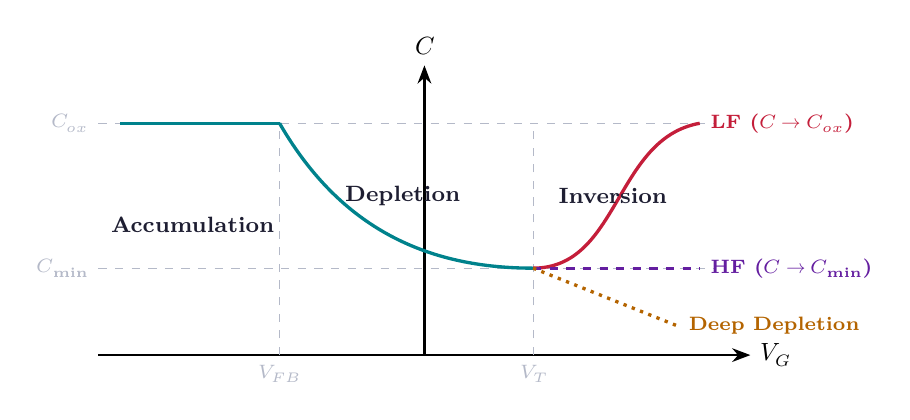
\begin{tikzpicture}[scale=0.92]
  \draw[-Stealth, thick] (-4.5, 0) -- (4.5, 0) node[right, font=\small] {$V_G$};
  \draw[-Stealth, thick] (0, 0) -- (0, 4.0) node[above, font=\small] {$C$};

  % Coordinates
  \coordinate (Cox) at (-4.0, 3.2);
  \coordinate (VFB) at (-2.0, 0);
  \coordinate (VT) at (1.5, 0);

  % Ticks
  \draw[dashed, color=mgframe] (-2.0, 0) node[below, font=\scriptsize] {$V_{FB}$} -- (-2.0, 3.2);
  \draw[dashed, color=mgframe] (1.5, 0) node[below, font=\scriptsize] {$V_T$} -- (1.5, 3.2);
  \draw[dashed, color=mgframe] (-4.5, 3.2) node[left, font=\scriptsize\bfseries\color{mydark}] {$C_{ox}$} -- (4.0, 3.2);
  \draw[dashed, color=mgframe] (-4.5, 1.2) node[left, font=\scriptsize\bfseries\color{mydark}] {$C_{\text{min}}$} -- (4.0, 1.2);

  % Accumulation Flat region
  \draw[very thick, color=myteal] (-4.2, 3.2) -- (-2.0, 3.2);

  % Depletion drop
  \draw[very thick, color=myteal] (-2.0, 3.2) to[out=-60, in=180] (1.5, 1.2);

  % Low-frequency recovery to Cox
  \draw[very thick, color=myred] (1.5, 1.2) to[out=0, in=-170] (3.8, 3.2) node[right, font=\scriptsize\bfseries\color{myred}] {LF ($C \to C_{ox}$)};

  % High-frequency flat at Cmin
  \draw[very thick, dashed, color=mypurple] (1.5, 1.2) -- (3.8, 1.2) node[right, font=\scriptsize\bfseries\color{mypurple}] {HF ($C \to C_{\text{min}}$)};

  % Deep depletion
  \draw[very thick, dotted, color=myamber] (1.5, 1.2) -- (3.5, 0.4) node[right, font=\scriptsize\bfseries\color{myamber}] {Deep Depletion};

  \node[font=\footnotesize\bfseries\color{mydark}] at (-3.2, 1.8) {Accumulation};
  \node[font=\footnotesize\bfseries\color{mydark}] at (-0.3, 2.2) {Depletion};
  \node[font=\footnotesize\bfseries\color{mydark}] at (2.6, 2.2) {Inversion};
\end{tikzpicture}
\end{tcolorbox}

% ===============================================================================
\section{MOSFET Operation and I-V Characteristics}
% ===============================================================================

The MOSFET is a four-terminal, voltage-controlled majority carrier field-effect transistor. By utilizing heavily doped Source and Drain regions that act as reservoirs of mobile electrons, the inversion channel can be modulated instantly, bypassing the slow thermal generation limit of the MOS capacitor.

\subsection{Operating Regimes of an n-Channel Enhancement MOSFET}
\begin{enumerate}[label=\arabic*., leftmargin=*]
  \item \textbf{Cut-off Region ($V_{GS} < V_T$):}
  No continuous inversion channel connects the source and drain. The drain-to-source path comprises two back-to-back p-n junctions ($n^+\text{--}p\text{--}n^+$). Ideal current $I_D = 0$. (In practice, subthreshold diffusion current flows: $I_D \propto \exp\left(\frac{V_{GS} - V_T}{n V_T}\right)$).

  \item \textbf{Linear / Triode Region ($V_{GS} \ge V_T$ and $V_{DS} < V_{GS} - V_T$):}
  An unbroken conducting channel exists from source to drain. The inversion charge density decreases smoothly from source ($Q_n(0) = -C_{ox}(V_{GS} - V_T)$) to drain ($Q_n(L) = -C_{ox}(V_{GS} - V_T - V_{DS})$). Integrating drift current:
  \begin{equation}
    I_D = \mu_n C_{ox} \frac{W}{L} \left[ (V_{GS} - V_T) V_{DS} - \frac{1}{2} V_{DS}^2 \right]
  \end{equation}
  For small $V_{DS} \ll 2(V_{GS} - V_T)$, the $V_{DS}^2$ term is negligible, and the MOSFET acts as a linear \textbf{voltage-controlled resistor}:
  \begin{equation}
    r_{DS} = \left(\frac{\partial I_D}{\partial V_{DS}}\right)^{-1} = \frac{1}{\mu_n C_{ox} \frac{W}{L} (V_{GS} - V_T)}
  \end{equation}

  \item \textbf{Pinch-Off and Saturation Region ($V_{GS} \ge V_T$ and $V_{DS} \ge V_{DS,\text{sat}} = V_{GS} - V_T$):}
  When $V_{DS}$ reaches the \textbf{saturation voltage} $V_{DS,\text{sat}} = V_{GS} - V_T$, the inversion layer charge at the drain end drops to zero ($Q_n(L) = 0$). This point is called \textbf{pinch-off}.
  \begin{itemize}
    \item Any further increase in $V_{DS}$ cannot increase the voltage drop across the remaining channel; the excess voltage $(V_{DS} - V_{DS,\text{sat}})$ is dropped across the high-field drain depletion region.
    \item Electrons reaching the pinch-off point are swept across the depletion space by the high electric field into the drain.
    \item Substituting $V_{DS} = V_{GS} - V_T$ yields the square-law saturation equation:
  \end{itemize}
  \begin{equation}
    I_{D,\text{sat}} = \frac{1}{2} \mu_n C_{ox} \frac{W}{L} (V_{GS} - V_T)^2
  \end{equation}
\end{enumerate}

\subsection{Channel Length Modulation (CLM)}
In the saturation region, as $V_{DS}$ increases past $V_{DS,\text{sat}}$, the pinch-off point migrates slightly toward the source. The effective channel length becomes $L_{\text{eff}} = L - \Delta L$. Because $I_D \propto 1/L_{\text{eff}}$, current rises slightly with $V_{DS}$:

\begin{tcolorbox}[formulabox, title={\textbf{MOSFET Saturation Current with Channel Length Modulation}}]
\begin{equation}
  I_D = \frac{1}{2} \mu_n C_{ox} \frac{W}{L} (V_{GS} - V_T)^2 \left( 1 + \lambda V_{DS} \right)
\end{equation}
where $\lambda = \frac{1}{V_A}$ is the \textbf{channel length modulation parameter} ($\text{V}^{-1}$), and $V_A$ is the MOSFET Early voltage ($V_A \propto L$).
\end{tcolorbox}

% ===============================================================================
\section{Small Signal Models of the MOS Transistor}
% ===============================================================================

\subsection{Low-Frequency Small-Signal Model Parameters}
Around a DC operating point ($V_{GS}, V_{DS}, V_{BS}, I_D$) in the saturation region:

\begin{enumerate}[label=\arabic*., leftmargin=*]
  \item \textbf{Transconductance ($g_m$):} Relates drain current variation to gate-to-source voltage changes:
  \begin{tcolorbox}[formulabox, title={\textbf{Three Equivalent Formulas for Transconductance $g_m$}}]
  \begin{equation}
    g_m = \left.\frac{\partial I_D}{\partial V_{GS}}\right|_{V_{DS}} = \mu_n C_{ox} \frac{W}{L} (V_{GS} - V_T) = \sqrt{2 \mu_n C_{ox} \frac{W}{L} I_D} = \frac{2 I_D}{V_{GS} - V_T}
  \end{equation}
  \end{tcolorbox}

  \item \textbf{Body Transconductance ($g_{mb}$):} Accounts for substrate voltage modulation via the body effect:
  \begin{equation}
    g_{mb} = \left.\frac{\partial I_D}{\partial V_{BS}}\right| = \left(\frac{\partial I_D}{\partial V_T}\right) \left(-\frac{\partial V_T}{\partial V_{SB}}\right) = \frac{\gamma}{2\sqrt{2\phi_F + V_{SB}}} g_m = \eta g_m
  \end{equation}
  where $\eta = \frac{g_{mb}}{g_m} \approx 0.1\text{--}0.25$.

  \item \textbf{Output Resistance ($r_o$):} Arises from channel length modulation:
  \begin{equation}
    r_o = \left.\left(\frac{\partial I_D}{\partial V_{DS}}\right)^{-1}\right|_{V_{GS}} = \frac{1}{\lambda I_D} = \frac{V_A}{I_D}
  \end{equation}
\end{enumerate}

\begin{tcolorbox}[tikzbox, title={Complete Small-Signal Equivalent Circuit of MOSFET (High-Frequency)}]
\centering
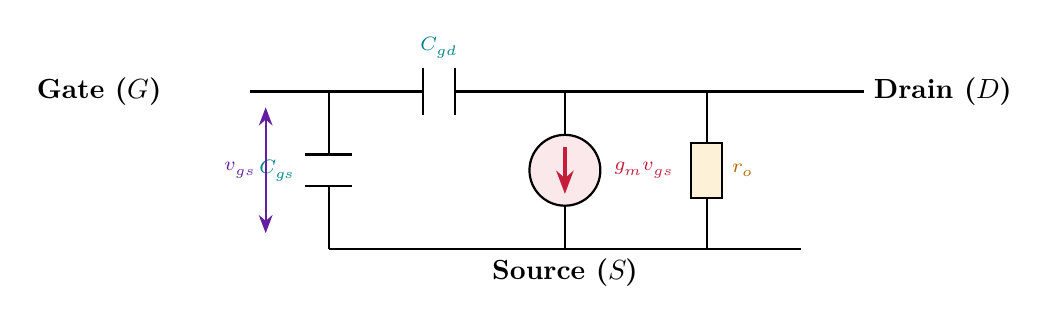
\begin{tikzpicture}[scale=1.0]
  % Gate terminal
  \node[left, font=\normalsize\bfseries] at (-4.0, 2.0) {Gate ($G$)};
  \draw[thick] (-3.0, 2.0) -- (-2.0, 2.0);

  % Source terminal (bottom ground line)
  \draw[thick] (-2.0, 0) -- (4.0, 0);
  \node[below, font=\normalsize\bfseries] at (1.0, 0) {Source ($S$)};

  % Cgs capacitor
  \draw[thick] (-2.0, 2.0) -- (-2.0, 1.2);
  \draw[thick] (-2.3, 1.2) -- (-1.7, 1.2);
  \draw[thick] (-2.3, 0.8) -- (-1.7, 0.8);
  \draw[thick] (-2.0, 0.8) -- (-2.0, 0);
  \node[left, font=\scriptsize\bfseries\color{myteal}] at (-2.3, 1.0) {$C_{gs}$};

  % vgs label
  \draw[Stealth-Stealth, thick, color=mypurple] (-2.8, 1.8) -- (-2.8, 0.2) node[midway, left, font=\scriptsize\bfseries] {$v_{gs}$};

  % Cgd bridging to Drain
  \draw[thick] (-2.0, 2.0) -- (-0.8, 2.0);
  \draw[thick] (-0.8, 2.3) -- (-0.8, 1.7);
  \draw[thick] (-0.4, 2.3) -- (-0.4, 1.7);
  \draw[thick] (-0.4, 2.0) -- (4.0, 2.0);
  \node[above, font=\scriptsize\bfseries\color{myteal}] at (-0.6, 2.3) {$C_{gd}$};

  % Dependent current source gm * vgs
  \draw[thick] (1.0, 2.0) -- (1.0, 1.45);
  \draw[thick, fill=hdrred] (1.0, 1.0) circle (0.45);
  \draw[-Stealth, very thick, color=myred] (1.0, 1.3) -- (1.0, 0.7);
  \node[right, font=\scriptsize\bfseries\color{myred}] at (1.5, 1.0) {$g_m v_{gs}$};
  \draw[thick] (1.0, 0.55) -- (1.0, 0);

  % Output resistor ro
  \draw[thick] (2.8, 2.0) -- (2.8, 1.35);
  \draw[thick, fill=hdramber] (2.6, 0.65) rectangle (3.0, 1.35);
  \node[right, font=\scriptsize\bfseries\color{myamber}] at (3.0, 1.0) {$r_o$};
  \draw[thick] (2.8, 0.65) -- (2.8, 0);

  % Drain terminal
  \draw[thick] (4.0, 2.0) -- (4.8, 2.0);
  \node[right, font=\normalsize\bfseries] at (4.8, 2.0) {Drain ($D$)};
\end{tikzpicture}
\end{tcolorbox}

\subsection{Unity-Gain Cut-Off Frequency (\texorpdfstring{$f_T$}{fT})}
The transition frequency $f_T$ is the frequency at which the short-circuit AC current gain of the common-source MOSFET drops to unity ($|i_d / i_g| = 1$):

\begin{tcolorbox}[formulabox, title={\textbf{Unity-Gain Cut-Off Frequency}}]
\begin{equation}
  f_T = \frac{g_m}{2\pi (C_{gs} + C_{gd})} \approx \frac{\mu_n C_{ox} \frac{W}{L} (V_{GS} - V_T)}{2\pi \left(\frac{2}{3} W L C_{ox}\right)} = \frac{3 \mu_n (V_{GS} - V_T)}{4\pi L^2}
\end{equation}
\textbf{Scaling Law:} $f_T \propto 1/L^2$. Reducing physical channel length $L$ yields a quadratic increase in operating speed and device bandwidth.
\end{tcolorbox}

\newpage
% ===============================================================================
% MANDATORY QUICK REVISION PAGE
% ===============================================================================
\begin{center}
  {\large\bfseries\color{myred} Quick Revision --- Module 3}\\[3pt]
  {\small\color{mydark} MOSFET Physics, C-V \& Small Signal Models $|$ EC301}
\end{center}
\noindent{\color{myred}\rule{\linewidth}{1.2pt}}
\vspace{4pt}

\begin{tcolorbox}[formulabox, title={\textbf{Key Formulas and Metrics at a Glance}}]
\renewcommand{\arraystretch}{1.35}
\begin{tabularx}{\linewidth}{B{5.0cm} X}
Oxide Capacitance per Area & $C_{ox} = \frac{\epsilon_{ox}}{t_{ox}}$ \\[4pt]
Flat-Band Voltage ($V_{FB}$) & $V_{FB} = \Phi_{ms} - \frac{Q_{ox}}{C_{ox}}$ \\[4pt]
Threshold Voltage ($V_{T0}$) & $V_{T0} = V_{FB} + 2\phi_F + \frac{\sqrt{4q\epsilon_s N_A \phi_F}}{C_{ox}}$ \\[4pt]
Body Effect Threshold Shift & $V_T = V_{T0} + \gamma \left(\sqrt{2\phi_F + V_{SB}} - \sqrt{2\phi_F}\right)$ \\[4pt]
Linear Region Drain Current & $I_D = \mu_n C_{ox} \frac{W}{L} \left[(V_{GS}-V_T)V_{DS} - \frac{1}{2}V_{DS}^2\right]$ \\[4pt]
Saturation Drain Current & $I_{D,\text{sat}} = \frac{1}{2}\mu_n C_{ox}\frac{W}{L}(V_{GS}-V_T)^2(1+\lambda V_{DS})$ \\[4pt]
Transconductance ($g_m$) & $g_m = \mu_n C_{ox}\frac{W}{L}(V_{GS}-V_T) = \sqrt{2\mu_n C_{ox}\frac{W}{L}I_D}$ \\[4pt]
Output Resistance ($r_o$) & $r_o = \frac{1}{\lambda I_D} = \frac{V_A}{I_D}$ \\[4pt]
Unity-Gain Frequency ($f_T$) & $f_T \approx \frac{g_m}{2\pi C_{gs}} \approx \frac{3\mu_n(V_{GS}-V_T)}{4\pi L^2}$ \\[4pt]
Maximum Depletion Width & $W_{\text{max}} = \sqrt{\frac{4\epsilon_s \phi_F}{q N_A}}$ \\[4pt]
\end{tabularx}
\end{tcolorbox}

\begin{tcolorbox}[defbox, title={\textbf{One-Line Definitions}}]
\begin{itemize}[leftmargin=*, itemsep=2pt, topsep=0pt]
  \item \textbf{Flat-Band Voltage ($V_{FB}$):} Gate voltage required to negate work-function differences and oxide charges, making bands flat.
  \item \textbf{Strong Inversion:} State where surface potential $\psi_s \ge 2\phi_F$, creating an electron sheet equal to bulk hole doping.
  \item \textbf{Pinch-Off:} Phenomenon where inversion channel charge at the drain vanishes when $V_{DS} \ge V_{GS} - V_T$.
  \item \textbf{Body Effect:} Increase in threshold voltage caused by applying a reverse bias between source and body substrate.
  \item \textbf{Channel Length Modulation:} Shortening of the effective channel length under high $V_{DS}$, producing finite output resistance.
  \item \textbf{Transconductance ($g_m$):} Rate of change of drain current with respect to gate-source voltage at constant $V_{DS}$.
  \item \textbf{Transition Frequency ($f_T$):} Frequency at which the small-signal short-circuit current gain drops to unity ($0\,\text{dB}$).
\end{itemize}
\end{tcolorbox}

\begin{tcolorbox}[exambox, title={\textbf{Frequently Asked / Viva Questions}}]
\begin{enumerate}[topsep=0pt, label=\textbf{Q\arabic*.}, itemsep=5pt]
  \item \Q{Why does the high-frequency C-V curve of an MOS capacitor remain at $C_{\text{min}}$ in inversion while the low-frequency curve recovers to $C_{ox}$?}
    In an isolated MOS capacitor, minority electrons can only be supplied via thermal generation-recombination across the bandgap, which is slow ($\tau \sim 0.01\text{--}0.1\,\text{s}$). At high frequencies ($f \ge 100\,\text{kHz}$), minority electrons cannot follow the AC signal, so the depletion layer capacitance $C_{\text{dep,max}}$ remains in series with $C_{ox}$, locking total capacitance at $C_{\text{min}}$. At low frequencies ($f \le 100\,\text{Hz}$), minority carriers respond, shielding the silicon bulk and restoring $C = C_{ox}$.
  \item \Q{Why does a MOSFET invert instantaneously while a standalone MOS capacitor takes significant time?}
    A MOSFET has heavily doped $n^+$ Source and Drain regions immediately adjacent to the channel, providing an abundant reservoir of electrons that can flow into the channel within picoseconds, whereas an MOS capacitor must wait for slow thermal EHP generation.
  \item \Q{What is the physical condition for the onset of strong inversion?}
    The surface potential must equal twice the bulk Fermi potential: $\psi_s = 2\phi_F = 2 V_T \ln(N_A / n_i)$. At this potential, the surface electron concentration $n_s = n_i e^{(\psi_s - \phi_F)/V_T}$ equals the substrate acceptor concentration $N_A$.
  \item \Q{Explain the physical mechanism of the Body Effect in a MOSFET.}
    Applying a reverse substrate bias ($V_{SB} > 0$) widens the depletion layer beneath the gate, exposing additional negative acceptor ions ($-q N_A$). The gate voltage must support this additional depletion charge before creating the inversion layer, thereby increasing $V_T$.
  \item \Q{What is Channel Length Modulation (CLM) and what is its effect on amplifier gain?}
    In saturation, high $V_{DS}$ shifts the pinch-off point toward the source, decreasing effective channel length $L_{\text{eff}} = L - \Delta L$. This causes drain current to increase with $V_{DS}$, giving the MOSFET a finite output resistance $r_o = 1/(\lambda I_D)$ and limiting maximum intrinsic voltage gain $A_{v0} = g_m r_o$.
  \item \Q{Compare enhancement-mode and depletion-mode MOSFETs.}
    Enhancement-mode MOSFETs have no physical channel at $V_{GS} = 0$ (normally OFF) and require $V_{GS} > V_T > 0$ to conduct. Depletion-mode MOSFETs have an implanted physical channel at $V_{GS} = 0$ (normally ON) and require a negative gate voltage $V_{GS} < V_T < 0$ to deplete the channel and turn off.
  \item \Q{Why is an n-channel MOSFET faster and smaller than a p-channel MOSFET for the same drive current?}
    Electron mobility in Silicon ($\mu_n \approx 1350\,\text{cm}^2/\text{V}\cdot\text{s}$) is nearly three times higher than hole mobility ($\mu_p \approx 480\,\text{cm}^2/\text{V}\cdot\text{s}$). To achieve equal current ($I_D \propto \mu W/L$), a PMOS device must be designed with roughly $2.5\text{--}3$ times greater width $W$, which increases parasitic capacitance and area.
  \item \Q{How does the unity-gain frequency $f_T$ depend on MOSFET gate length?}
    $f_T \approx \frac{3\mu_n(V_{GS}-V_T)}{4\pi L^2} \propto \frac{1}{L^2}$. It scales inversely with the square of the channel length, which has been the primary technological driving force behind semiconductor feature scaling.
  \item \Q{What is deep depletion in an MOS capacitor?}
    Deep depletion occurs when a rapid positive voltage ramp is applied to the gate so fast that no inversion electrons can generate. The depletion layer expands past $W_{\text{max}}$, and capacitance continues dropping below $C_{\text{min}}$. This state is utilized in CCD image sensors.
  \item \Q{What is the transconductance parameter $k_n'$ and device transconductance parameter $k_n$?}
    Process transconductance parameter $k_n' = \mu_n C_{ox}$ ($\text{A/V}^2$), which depends purely on fabrication technology. Device transconductance parameter $k_n = k_n' (W/L) = \mu_n C_{ox} (W/L)$, which depends on circuit designer sizing.
\end{enumerate}
\end{tcolorbox}

\begin{tcolorbox}[tikzbox, title={Comparison of BJT and MOSFET Device Characteristics}]
\centering
\renewcommand{\arraystretch}{1.45}
\begin{tabularx}{\linewidth}{|B{3.2cm}|Y|Y|}
\hline
\multicolumn{1}{|c|}{\textbf{Parameter}} & \multicolumn{1}{c|}{\textbf{Bipolar Junction Transistor (BJT)}} & \multicolumn{1}{c|}{\textbf{MOSFET}} \\
\hline
Operating Principle & Current-controlled device ($I_C = \beta I_B$) & Voltage-controlled device ($I_D \propto V_{GS}^2$) \\
\hline
Carrier Type & Bipolar (both electrons and holes participate) & Unipolar (majority carriers only in channel) \\
\hline
Input Impedance & Low to moderate ($1\text{--}10\,\text{k}\Omega$ in active mode) & Extremely high ($> 10^{12}\,\Omega$, isolated gate oxide) \\
\hline
Input Current & Continuous DC base current $I_B = I_C / \beta$ & Zero static gate current ($I_G \approx 0$) \\
\hline
Temperature Coefficient & Negative ($\text{NTC}$): prone to thermal runaway & Positive ($\text{PTC}$): thermally self-limiting \\
\hline
Noise Figure & Low $1/f$ flicker noise; higher shot noise & Higher flicker noise ($1/f$ interface states) \\
\hline
Fabrication Density & Moderate; requires isolation wells & Extremely high; self-aligned planar process \\
\hline
Primary Applications & High-speed RF, precision analog, linear power & Digital VLSI, microprocessors, CMOS logic, power \\
\hline
\end{tabularx}
\end{tcolorbox}

\end{document}
